\graphicspath{{chapters/greco/images/level6/}}

\subsection{GRECO Level 6 Cuts}
Unlike previous levels, the GRECO L6 does not rely on a trained boosted decision tree.
The choice was made to use solely stright cuts due to initial concerns about the significantly limited background simulation.
Such a limitation could lead to overtraining, a situation difficult to test with so few simulated events.

Instead, there are effectively two types of cuts used in the GRECO L6:
those that deal, directory or indirectly, with removing accidental triggers and those that focus on the starting containment of events in the DeepCore fiducial volume.

\subsubsection{Fill-Ratio at L6}
\begin{figure}[h]
	\centering
		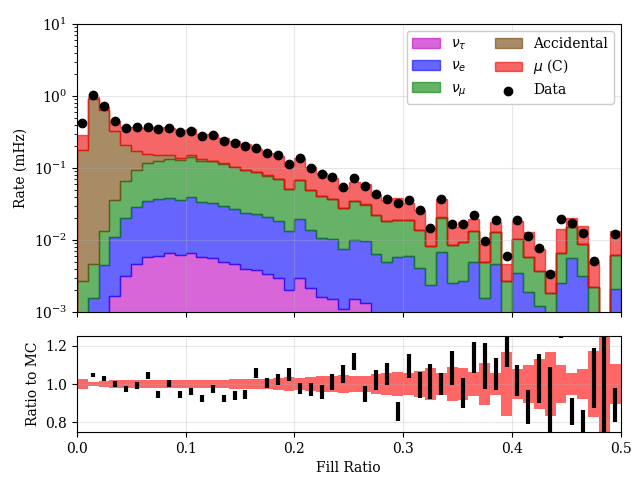
\includegraphics[width=2.5in]{FillRatio.png}
		\caption[Fill-Ratio]{The fill-ratio distribution. Note the excess of noise triggers at low values. A cut is applied at 0.05 to remove these accidental triggers.}
	\label{fig:fill-ratio}
\end{figure}

A continuing thread of the event selection deals with understanding and removing events caused by detector noise triggering in the DeepCore fiducial volume.
While the rate of these accidental triggers is low at this stage relative to the rate at L3, they form an important background to the remaining set of neutrino events.
In order to limit their effect, various cuts were investigated for the potential to separate signal neutrinos from the accidental background.

The most promising cut was discovered to be a remnant of earlier AMANDA processing efforts at separating atmospheric muon background and cascade signal events.
This cut, called \emph{Fill-Ratio}, looks at the topology and compactness of hits within an event.

Fill-Ratio requires a reconstructed vertex and pulse series.
In the case of the GRECO L6, the first hit position in DeepCore within a 7.5 microsecond STW cleaned pulse series is used as an approximate event vertex.
The hit series chosen, TWSRTOfflinePulses, offers some cleaning as well.

Once a vertex and pulse series are provided, a radius is computed.
Many options are available for the caclulation of different radii, although the most effective for this event selection is the mean distance from the vertex.

\begin{equation}
	\bar{r}_{Fill-Ratio} = A \left|\frac{\sum_i^{npulses} \left(\vec{x_i}-\vec{x}_{vertex}\right)}{npulses}\right|
\end{equation}

where $A$ is a configurable scale factor. 
Within this radius, the algorithm indentifies all contained DOMs.
The cut value is then given by the ratio of contained DOMs observing a pulse to the total number of contained DOMs.

\begin{equation}
	f = \frac{\sum_i^{ncont} \left(|\vec{r_i}\right|<\bar{r}_{Fill-Ratio} \;\&\; Q_i>0}{\sum_j^{ncont} \left(|\vec{r_j}\right|<\bar{r}_{Fill-Ratio}}
\end{equation}

This effectively results in a measure of the compactness of a hypothetical cascade, where we expect the resulting hit distribution to be approximately spherically symmetric.
In the case of an extended track, this parameter will yield a larger value of $\bar{r}_{Fill-Ratio}$.
The larger value, in turn, will result in a higher number of contained DOMs and, therefore, a lower value of this parameter.
This is particularly true in the case of accidental triggers, where we have no reason to expect a compact hit distribution a priori.
Using a loose choice of $A$ of 1.6, we concentrate the accidental triggers in just a few bins close to $f$=0.

The observed separation at a value of 0.05 allows up to one order of magnitude of reduction in the rate of accidental triggers with a relatively small reduction in signal rate of approximately 10\%.


\subsubsection{The L6 NChannel Cut}
\begin{figure}[h]
	\centering
		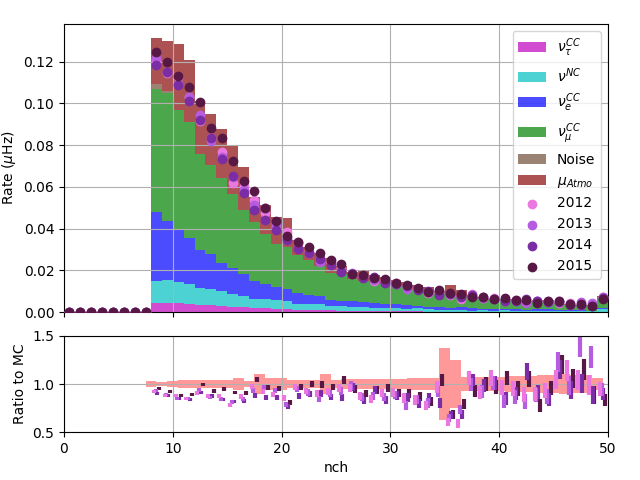
\includegraphics[width=2.5in]{nch.png}
		\caption[The NChannel Distribution]{The number of channels in a cleaned hit series. At least 8 hits are required for the reconstruction.}
	\label{fig:nchannel}
\end{figure}

The reconstruction chosen for the final stages of this event selection attempt to reconstruct a total of eight variables: the position ($x$, $y$, $z$), time ($t$), the direction ($\theta$, $\phi$), the energy deposited in the proposed hadronic cascade ($E_{casc}$), and the track length ($L$).
The reconstruction, described in more detail in \ref{subsec:pegleg_reco}, uses information both from the hit DOMs as well as unhit DOMs in order to constrain the reconstructed parameters.
In order to constrain all parameters using observed hits, as opposed to relying on information from unhit DOMs, the decision was made to process only DOMs possessing more than 8 hits in the SRTTWOfflinePulsesDC pulse series.

In addition to providing a more robust reconstruction, the additional cut on the required number of hits further reduces the expected rate of accidental triggers in the detector by another order of magnitude.
These accidental triggers make up about 0.3\% of events in the sample following these cuts.


\label{subsubsec:corridorcut}
\subsubsection{CorridorCut}
\begin{figure}[h]
	\centering
		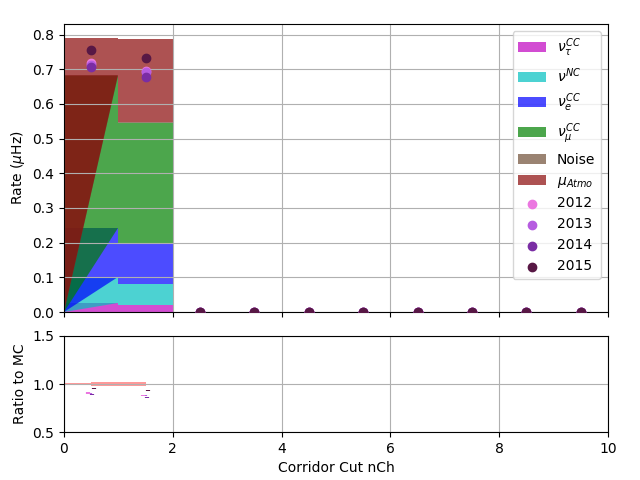
\includegraphics[width=2.5in]{Corridor_Cut_nCh.png}
		\caption[CorridorCut Distribution]{The number of channels discovered along one of the various "corridors" in the detector. Events with at least two hits discovered along a corridor are removed.}
	\label{fig:corridorcut}
\end{figure}

At later cut levels, atmospheric muons continue to be problematic.
Unfortunately muons at this level tend to be difficult to identify muons based on many parameters.
Indeed, any muons that were easily identifiable have been removed already by this stage of the selection.

In the past, minimum-ionizing muons were discovered to be leaking into the DeepCore fiducial volume along \emph{corridors}, lines connecting the inner part of the detector to the outer edge without crossing any strings.
These events pass between strings and leave little trace in the form of coincident hits in the outer detector.

In order to identify these muons, a cut was developed to look specifically along these pre-defined corridors for hits potentially correlated with pulses in DeepCore.
Due to the effects of random detector noise, a cut limiting the number of discovered corridor hits to 0 would result in a significant loss of signal events.
Instead, one hit is allowed, with two or more discovered DOMs leading to the removal of the event from further processing.
At this stage, there are few events due to atmospheric muons with detectable energy in the veto, resulting in the removal of very few events.



\subsubsection{FiniteReco Starting Containment}
\begin{figure}{h}%
	\centering
		\subfloat[$\rho_{FiniteReco}$]{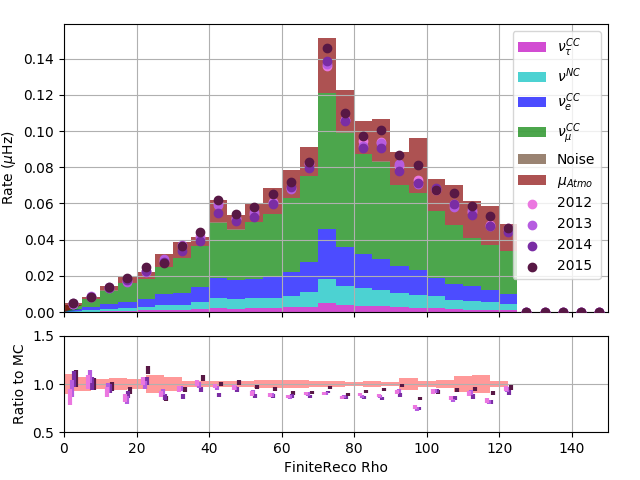
\includegraphics[width=2.3in]{FiniteReco_Rho.png}}%
		\subfloat[$Z_{FiniteReco}$]{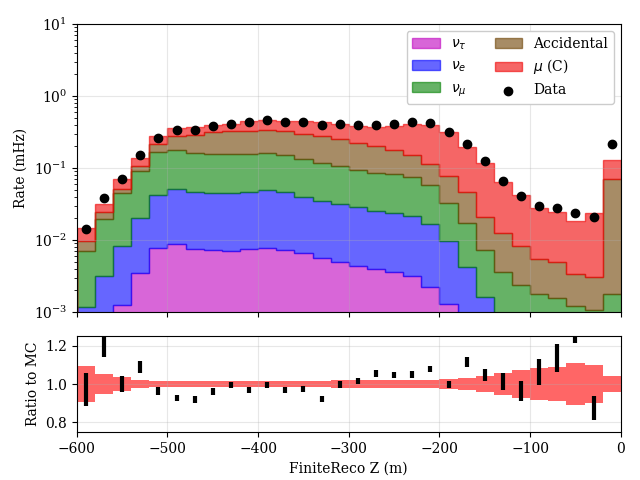
\includegraphics[width=2.3in]{FiniteReco_Z.png}}%
	\caption[The FiniteReco Containment Cuts]{The FiniteReco containment cuts. Note the exces of muons at the top and outer edge of the DeepCore fiducial volume.}%
	\label{fig:finitereco_cuts}%
\end{figure}

The SPE reconstruction used in L5 was created using an infinite muon hypothesis. 
In order to refine this reconstruction, the \emph{FiniteReco} algorithm is employed.

FiniteReco is a module that accepts a previous reconstruction and a given set of pulses.
The pulses are then used in a likelihood reconstruction in order to obtain estimates for the starting and stoppoing positions as well as the starting time for the given muon track.
The direction of the muon track remains unchanged.

The starting position of the resulting reconstructed particle may be used to estimate the interaction point of the particle.
\ref{fig:finitereco_zVsRho} shows the position of the reconstructed vertex in terms of depth and distance from the center of the volume.
If an event begins outside of the DeepCore fiducial volume, particularly if the event appears at the top of the fiducial volume, the event is likely to contain a muon and can be removed from the sample.
Cuts are applied at the positions shown, resulting in a significant reduction in the number of muon events expected at final level.

\begin{center}
\begin{table}
\begin{tabular}{cc}
    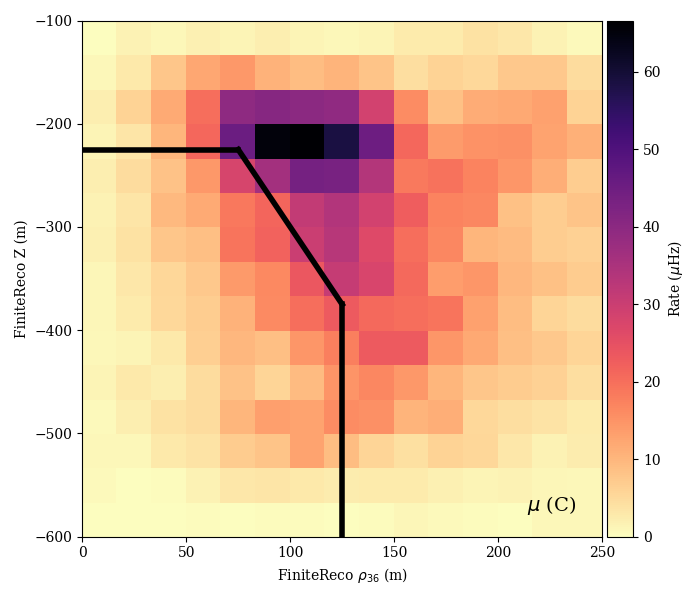
\includegraphics[width=0.45\linewidth]{z_rho_corsika.png} &  
    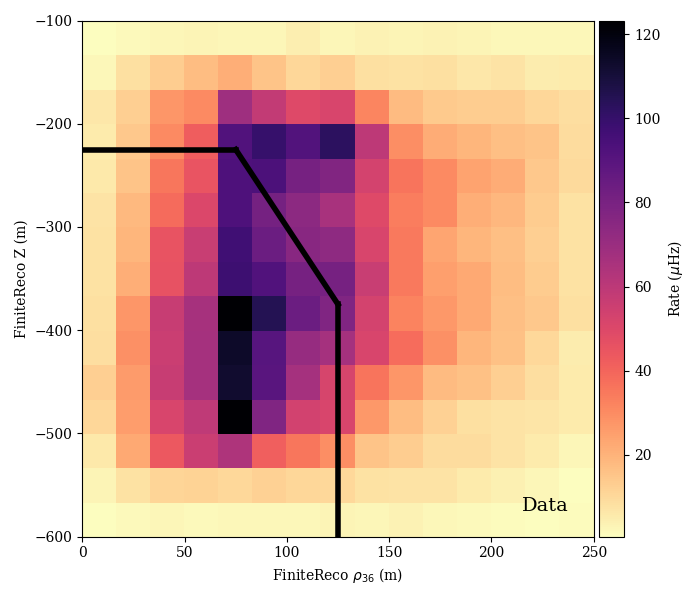
\includegraphics[width=0.45\linewidth]{z_rho_data.png} \\  

    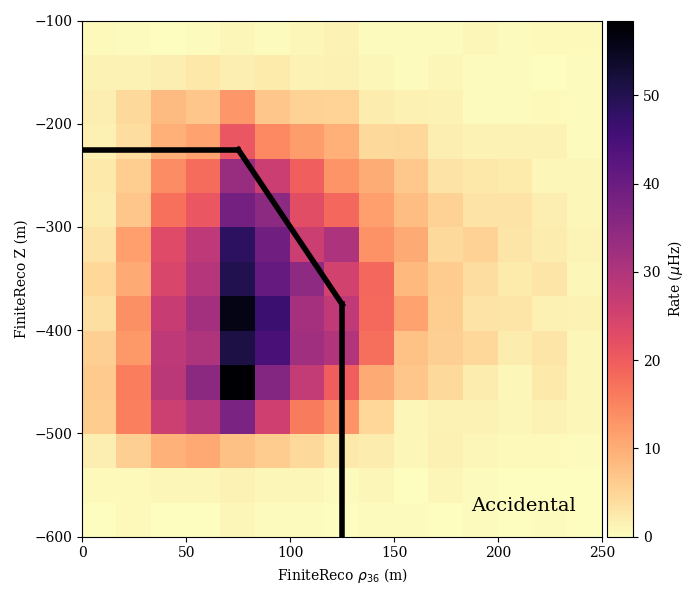
\includegraphics[width=0.45\linewidth]{z_rho_noise.png} &  
    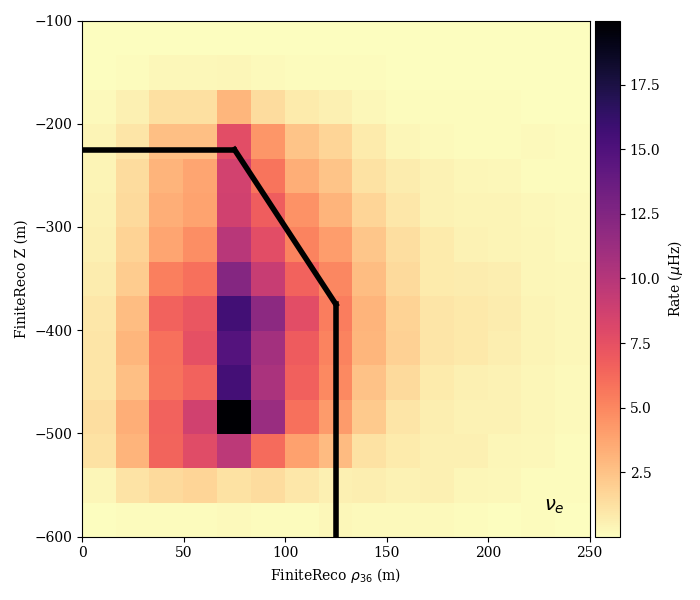
\includegraphics[width=0.45\linewidth]{z_rho_genie_nue.png} \\  

    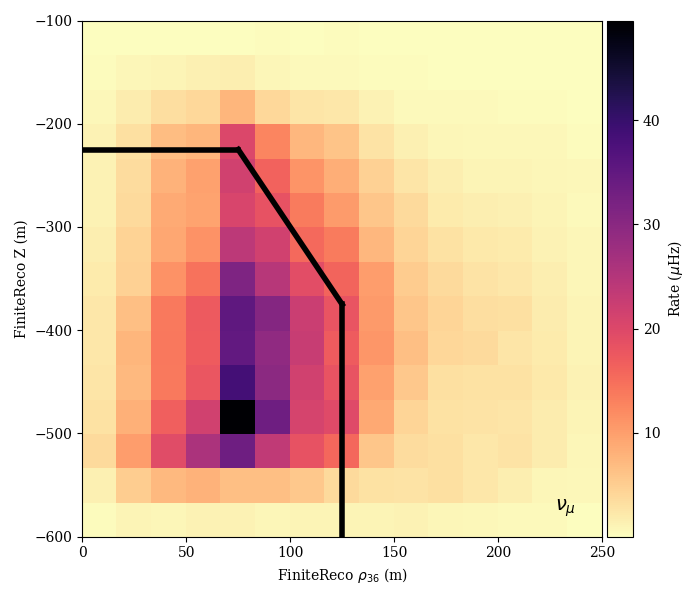
\includegraphics[width=0.45\linewidth]{z_rho_genie_numu.png} &  
    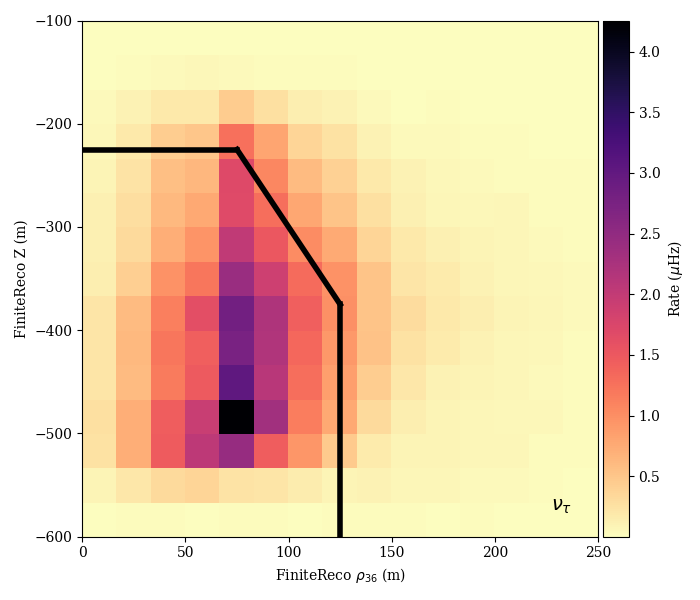
\includegraphics[width=0.45\linewidth]{z_rho_genie_nutau.png} \\ 
\end{tabular}
\label{fig:finitereco_zVsRho}
\caption{The FiniteReco containment cut for each of the channels. The cut itself is shown with the black line.}
\end{table}
\end{center}

